\chapter{Preliminaries and Related Work}\label{sec-preliminaries}

In this chapter, we first give a brief introduction on the GPU, and then review the related work on GPGPU as well as on MapReduce.


\section{Graphics Processing Units (GPUs)}

The GPU is an integral component of
modern computers, ranging from handheld devices to high-end servers.
GPUs are originally designed for gaming applications with fixed
hardware pipelines for rendering. Due to the high computation power
and rapidly improving programmability, they have recently become a
powerful co-processor for general purpose computing~\cite{Ailamaki2006}.
%For example, NVIDIA Tesla GPU series have been
%adopted to high performance computers and clusters~\cite{Tesla}. For
%more details on the GPU and its programming techniques, we refer the
%reader to a recent book edited by Nguyen~\cite{GPUGems}.


\begin{figure}[ht]
\centering
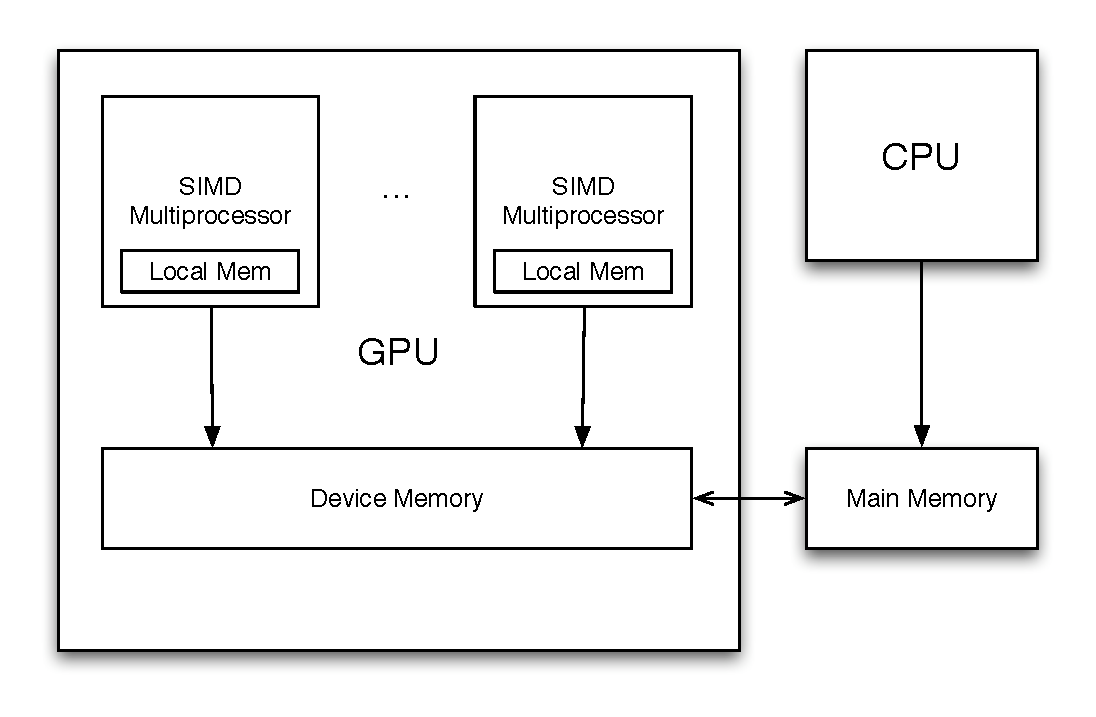
\includegraphics[width=0.65\textwidth]{figure/gpuarch.eps}
\caption{The many-core architecture model for GPUs}
\label{fig:manycore}
\end{figure}



%The major vendors such as NVIDIA and AMD provide similar programmable hardware pipelines, and develop similar programming frameworks.
As shown in Figure \ref{fig:manycore}, we model the GPU as a many-core processor, which
contains a number of SIMD multiprocessors.
Such a many-core model is common to both AMD and NVIDIA GPUs.
On the GPU board, there is a GRAM device memory.
The device memory has both a high bandwidth and a high access latency.
For example, the NVIDIA GTX280 GPU has an access latency of 400 to 600 cycles, and
the peak memory bandwidth between the device memory and the multiprocessors
is around 140 GB/second.

Both NVIDIA CUDA and AMD Brook+ expose a parallel programming model, which does not require programmers to have knowledge of the
graphics rendering pipeline. In this model, the system consists of a
{\em host} (a CPU), and one or more {\em devices} (GPUs).
GPUs are abstracted as massively data-parallel co-processors.
CUDA and Brook+ programmers write code using C/C++ syntax with extended keywords for kernel functions,
which are GPU programs to be executed on {\em devices}.

Programming frameworks such as CUDA and Brook+ greatly improve
the programmability of the GPU.
However, it is still a challenging task of developing efficient GPU programs for complex applications, such as those with MapReduce, because GPUs have a special-purpose co-processor architecture and are vendor-specific on the programming frameworks for complex applications.
\red{Although the newly introduced OpenCL~\cite{OPENCL} is an industry standard further hiding hardware details from users, Mars is at a higher level of abstraction.} OpenCL is a general-purpose programming language, with which Mars or other MapReduce frameworks can be developed.

\section{GPGPU}




GPGPU, or General Purpose Computation on GPUs, has recently emerged
in various applications, such as linear algebra~\cite{Jiang2005,Volkov2008}, embedded system design~\cite{Feng2007}, bioinformatics~\cite{Charalambous2005}, databases~\cite{Govindaraju2006,Govindaraju2004,He2008a}, machine learning~\cite{Chu2006}, and
distributed computing projects including Folding@home and Seti@home.
Recently, several GPGPU languages including AMD Brook+~\cite{BROOKPLUS} (extended from Brook~\cite{Buck2004}) and NVIDIA
CUDA~\cite{CUDA} have been proposed by GPU vendors. They usually
expose a general-purpose, massively multi-threaded computing
architecture and provide a programming environment similar to C/C++.
High-level programming frameworks such as Accelerator~\cite{Tarditi2006} and RapidMind~\cite{McCool2006} are also
developed to better facilitate GPGPU programming. These
programming frameworks require programmers to have knowledge of specific
programming models such as the stream programming model in Brook+~\cite{Buck2004}, or even more, knowledge of the GPU hardware
details. By contrast, we propose to develop a MapReduce framework accelerated with
GPUs to ease the development of a more complex class of data
processing tasks. It provides a uniform MapReduce interface no matter whether it runs on the GPU, on the CPU, or both.

We now briefly survey recent  work that developed GPGPU primitives as building blocks for various applications, in particular, those not covered in the survey by Owens et al~\cite{Owens2007}.
Sengupta et al.~\cite{Sengupta2007} proposed the segmented scan primitive.
He et al.~\cite{He2007} proposed a multi-pass scheme to optimize the scatter and the gather operations.
He et al.~\cite{He2008a} further developed a small set of primitives such as prefix sum and split for relational databases.
Additionally, CUDPP~\cite{CUDPP}, a CUDA library of data parallel primitives, was released for GPGPU computing.
These GPU-based primitives reduce the complexity of GPU programming.
However, even with the primitives, programmers need to write complex GPU code for data processing tasks.
By contrast, our work further simplifies GPU programming for MapReduce programmers by providing them with a higher level and more familiar interface than the primitives.

\red{This thesis focuses  on  accelerating  MapReduce  on  the  GPU,  and  provides  a  GPU-based MapReduce framework to developers. As in the original MapReduce,  it  is  up  to  developers'  choice  whether to  use  MapReduce  or  not  according  to the workload's computational characteristics. Recent studies \cite{Kerr2010}  have used data analysis techniques to categorize the computational characteristics of different workloads on the GPU. These techniques are helpful for developers to determine whether their workloads are suitable for Mars in
specific and the GPU in general.}

%Our previous study on Mars~\cite{He2008} implemented the MapReuduce framework on CUDA-enabled GPUs. This work extends the previous work in two major aspects. First, we extend the CUDA-only Mars to another large group of GPUs, so that it can run on both NVIDIA and AMD GPUs. Second, we use GPU-only Mars as a component to work with CPU-based Mars on a single machine, as well as with Hadoop in a distributed environment.

\section{MapReduce}
The MapReduce framework~\cite{Dean2008} is based on two primitives, Map and Reduce, from functional programming.
The general form is as follows:
\begin{quote}
\tab \bf{Map:} $(k_1, v_1) \rightarrow list(k_2, v_2)$.

\tab \bf{Reduce:} $(k_2, list(v_2)) \rightarrow list(k_3, v_3)$.
\end{quote}



The Map function takes an input key/value pair $(k_1, v_1)$ and outputs a list of intermediate key/value pairs $(k_2, v_2)$.
The Reduce function takes all values associated with the same key and produces a list of key/value pairs.
Programmers implement the application logic inside the Map function and the Reduce function.
The MapReduce runtime manages the parallel execution of these two functions.



The following pseudo code illustrates a program written using MapReduce.
This program counts the number of occurrences of each word in a collection of documents~\cite{Dean2008}.
In this program, {\em Map} and {\em Reduce} are implemented using two system-provided APIs, {\em EmitIntermediate} and {\em Emit}, respectively.

\begin{quote}
{\bf Map}(void *{\em doc}) \{ \\
1: {\bf for} each word {\em w} in {\em doc} \\
2: \hspace{3mm} {\bf EmitIntermediate}({\em w}, {\em 1}); // count each word once \\
\} \\
{\bf Reduce}(void *{\em word}, Iterator {\em values}) \{ \\
1: int {\em result} = 0; \\
2: {\bf for} each {\em v} in {\em values} \\
3: \hspace{3mm} {\em result} += {\em v}; \\
4: {\bf Emit}({\em word}, {\em result}); // output {\em word} and its count \\
\}
\end{quote}

%\begin{quote}
%\tab {\bf Map}(void *{\em doc}) \{ \\
%\tab 1: \tab {\bf for} each word {\em w} in {\em doc} \\
%\tab 2: \tab \tab {\bf EmitIntermediate}({\em w}, {\em 1}); // count each word once \\
%\tab \} \\
%\tab {\bf Reduce}(void *{\em word}, Iterator {\em values}) \{ \\
%\tab 1: \tab int {\em result} = 0; \\
%\tab 2: \tab {\bf for} each {\em v} in {\em values} \\
%\tab 3: \tab \tab {\em result} += {\em v}; \\
%\tab 4: \tab {\bf Emit}({\em word}, {\em result}); // output {\em word} and its count \\
%\tab \}
%\end{quote}

There have been several MapReduce implementations since MapReduce was proposed~\cite{Dean2008}.
Hadoop~\cite{HADOOP} is an open-source MapReduce implementation on clusters.
Based on Hadoop, Yang et al.~\cite{Yang2007} added the merge operation to MapReduce for the ease of relational databases operations.
Phoenix~\cite{Ranger2007} is an efficient MapReduce runtime system on multi-core CPUs.
Kruijf et al.~\cite{Kruijf2007} developed MapReduce on the Cell BE.
Yeung et al.~\cite{Yeung2008} implemented an FPGA-based MapReduce system.

\red{Let us briefly introduce the implementation of Phoenix~\cite{Ranger2007}. A key component in Phoenix is a scheduler, for buffer management and task distribution. The scheduler starts the Map stage by evenly dividing the input buffer into small chunks, and assigns the chunks to map workers dynamically. Each map worker runs in a CPU thread. The Reduce stage does not start until all Map tasks are done. The scheduler groups the intermediate output from the Map stage by key, and a Reduce worker processes values associated with the same key. Reduce tasks are assigned to workers dynamically. Each reduce worker maintains a static array for outputting results, and sorts this static array using insertion sort. Finally, the scheduler merges all output arrays of reduce workers into a single one. Because the output data size is not known in advance, the scheduler first allocates buffers with a default small size, and then resizes the buffer as needed.}


%Our previous work on Mars implemented MapReduce on CUDA-enabled GPUs~\cite{He2008}. 
Catanzaro et al.~\cite{Catanzaro2008}, developed another MapReduce system on the GPU, but it required programmers to be aware of GPU hardware details, such as thread configuration and memory hierarchy.
Finally, the Merge framework~\cite{Linderman2008}, focused on dynamically scheduling MapReduce tasks among multiple processors, dedicated to Intel products.
By contrast, Mars hides hardware details from programmers, and works on heterogeneous GPUs, a combination of CPU and GPU on a single machine, as well as a distributed system of multiple machines.

\newpage
